\documentclass[11pt,a4paper]{article}
\usepackage[utf8]{inputenc}
\usepackage[T1]{fontenc}
\usepackage[brazil]{babel}
\usepackage{lmodern}
\usepackage{amsmath,amssymb,amsthm}
\usepackage{graphicx}
\usepackage{booktabs}
\usepackage{array}
\usepackage[margin=2.5cm]{geometry}
\usepackage{listings}
\usepackage{xcolor}
\usepackage[hidelinks]{hyperref}
\usepackage{caption}
\usepackage{float}

\lstset{language=Python, basicstyle=\ttfamily\small, keywordstyle=\color{blue!60!black},
  commentstyle=\color{green!40!black}, stringstyle=\color{red!50!black},
  frame=single, framerule=0.3pt, breaklines=true, columns=fullflexible,
  literate={á}{{\'a}}1 {é}{{\'e}}1 {í}{{\'i}}1 {ó}{{\'o}}1 {ú}{{\'u}}1 {ã}{{\~a}}1
           {õ}{{\~o}}1 {ç}{{\c c}}1 {ê}{{\^e}}1 {â}{{\^a}}1 {ô}{{\^o}}1 {à}{{\`a}}1
           {ε}{{$\varepsilon$}}1 {²}{{$^2$}}1 {·}{{$\cdot$}}1}

\newtheorem{proposicao}{Proposição}
\newtheorem{observacao}{Observação}
\newcommand{\fl}{\operatorname{fl}}
\renewcommand{\Im}{\operatorname{Im}}
\renewcommand{\Re}{\operatorname{Re}}

\title{Diferenciação automática, passo complexo e diferenças finitas:\\
\large por que só os dois primeiros atingem o arredondamento unitário}
\author{Felipe M. Figueira \and Lucas Carvalhosa Lago}
\date{\small Seminário --- outubro de 2026}

\begin{document}
\maketitle

\begin{abstract}
Diferenças finitas aproximam derivadas por quocientes de diferenças e, em aritmética de ponto flutuante, estão sujeitas a um compromisso inevitável entre erro de truncamento e erro de cancelamento: o melhor erro alcançável com um método de ordem $p$ é da ordem de $u^{p/(p+1)}$, onde $u\approx1{,}1\times10^{-16}$ é o arredondamento unitário. Mostramos que o passo complexo elimina a subtração (e com ela o termo $u/h$), e que a diferenciação automática no modo direto, formalizada por números duais, elimina também o truncamento. Ambos atingem erro da ordem de $u$. O preço é pago em generalidade: o passo complexo exige funções analíticas implementadas com operações ``seguras'' para complexos; os duais exigem que todo o programa seja escrito em operações sobrecarregáveis. Implementamos uma classe \texttt{Dual} em Python e realizamos experimentos em NumPy, JAX e PyTorch que confirmam as previsões teóricas, e discutimos o custo $O(n)$ do modo direto para gradientes, contra o custo $O(1)$ do modo reverso.
\end{abstract}

\tableofcontents

%======================================================================
\section{Introdução}

Derivadas aparecem em toda parte em computação científica: métodos de Newton, otimização, análise de sensibilidade, treinamento de redes neurais e etc. Há quatro formas de obtê-las num computador: (i) derivação manual, (ii) derivação simbólica, (iii) aproximação numérica por diferenças finitas e (iv) diferenciação automática (AD). Este trabalho compara (iii) e (iv), com uma técnica intermediária, o \emph{passo complexo}~\cite{squire1998,martins2003}, que serve de ponte conceitual entre as duas.

A pergunta central é:

\begin{quote}
\emph{Por que diferenças finitas nunca atingem erro $u$, e o que exatamente o passo complexo e a AD fazem para atingi-lo? Qual é o custo em generalidade (tipos de $f$ aceitos) e em implementação?}
\end{quote}

\paragraph{Modelo de ponto flutuante.} Usamos o modelo padrão (IEEE-754): para $a,b$ números de máquina e $\circ\in\{+,-,\times,/\}$,
\begin{equation}
\fl(a\circ b) = (a\circ b)(1+\delta), \qquad |\delta|\le u = 2^{-53}\approx 1{,}11\times 10^{-16}
\end{equation}
em precisão dupla. Supomos também que a avaliação de $f$ é feita com erro relativo da ordem de $u$: $\hat f(x) = f(x)(1+\delta_f)$, $|\delta_f|\lesssim u$.\footnote{Na prática $|\delta_f|$ pode ser alguns múltiplos de $u$; isso muda constantes, não expoentes.}

Todo o código está no notebook \texttt{experimentos\_ad.ipynb}; as figuras deste relatório são geradas por ele.

%======================================================================
\section{Diferenças finitas: o compromisso truncamento $\times$ cancelamento}
\label{sec:fd}

\subsection{Diferença progressiva}
Por Taylor, $f(x+h) = f(x) + hf'(x) + \tfrac{h^2}{2}f''(\xi)$, logo
\begin{equation}
D_+(h) = \frac{f(x+h)-f(x)}{h} = f'(x) + \underbrace{\tfrac{h}{2}f''(\xi)}_{\text{truncamento}} .
\end{equation}
Em ponto flutuante, cada avaliação tem erro absoluto até $u|f|$. Como $f(x+h)\approx f(x)$, a subtração é exata (lema de Sterbenz) mas \emph{revela} esses erros: a diferença calculada tem erro absoluto de até $2u|f|$, que é dividido por $h$:
\begin{equation}
|\hat D_+(h) - f'(x)| \lesssim \frac{h}{2}|f''| + \frac{2u|f|}{h} .
\label{eq:erro-prog}
\end{equation}
Esse é o \textbf{cancelamento catastrófico}: os primeiros dígitos de $f(x+h)$ e $f(x)$ coincidem e se anulam, sobrando apenas os dígitos contaminados por arredondamento. Minimizando~\eqref{eq:erro-prog} em $h$:
\begin{equation}
h^\ast = 2\sqrt{\frac{u|f|}{|f''|}}, \qquad E(h^\ast) = 2\sqrt{u|f||f''|} = O(u^{1/2}).
\end{equation}

\subsection{Diferença centrada}
Subtraindo as expansões de $f(x\pm h)$, os termos pares se cancelam:
\begin{equation}
D_c(h) = \frac{f(x+h)-f(x-h)}{2h} = f'(x) + \frac{h^2}{6}f'''(x) + \frac{h^4}{120}f^{(5)}(x) + O(h^6).
\label{eq:centrada}
\end{equation}
O numerador tem erro de até $2u|f|$, dividido por $2h$, e portanto
\begin{equation}
E_c(h) \approx \frac{h^2}{6}|f'''| + \frac{u|f|}{h}, \qquad
h^\ast = \left(\frac{3u|f|}{|f'''|}\right)^{1/3}, \qquad E_c(h^\ast) = O(u^{2/3}).
\end{equation}

\subsection{Extrapolação de Richardson}
Combinando $D_c(h)$ e $D_c(h/2)$ para eliminar o termo $h^2$ de~\eqref{eq:centrada},
\begin{equation}
D_R(h) = \frac{4D_c(h/2)-D_c(h)}{3} = f'(x) - \frac{h^4}{480}f^{(5)}(x) + O(h^6).
\end{equation}
Os coeficientes amplificam o arredondamento: $\frac43\cdot\frac{2u|f|}{h} + \frac13\cdot\frac{2u|f|}{2h} = \frac{3u|f|}{h}$. Assim
\begin{equation}
E_R(h)\approx \frac{h^4}{480}|f^{(5)}| + \frac{3u|f|}{h}, \qquad h^\ast = \left(\frac{360\,u|f|}{|f^{(5)}|}\right)^{1/5},\qquad E_R(h^\ast)=O(u^{4/5}).
\end{equation}

\subsection{O resultado geral}
\begin{observacao}
Seja $D_p(h)$ uma fórmula de diferenças finitas de ordem $p$ para $f'(x)$, isto é, uma combinação $\frac1h\sum_k c_k f(x+kh)$ com $\sum_k c_k=0$ e erro de truncamento $C_ph^p$ e supondo $f^{(p+1)}(x)$ diferente de $0$. Então o erro total satisfaz $E(h)\approx C_ph^p + K_pu|f|/h$, cujo mínimo é
\[
E(h^\ast)  \sim u^{p/(p+1)} \quad\text{com}\quad h^\ast \sim u^{1/(p+1)}.
\]
Como $p/(p+1)<1$ para todo $p$ finito, nenhuma fórmula de diferenças finitas atinge erro $O(u)$.
\end{observacao}

A condição $\sum_kc_k=0$ é exatamente o que torna a fórmula exata para constantes --- e é ela que obriga a subtrair valores próximos de $f$. \emph{O termo $u/h$ é consequência inevitável da subtração.} Aumentar a ordem empurra o expoente para perto de 1, mas as constantes $K_p$ crescem e o expoente nunca chega lá. Além disso, para $h<u|x|$ tem-se $\fl(x+h)=x$ e a fórmula devolve exatamente zero.

%======================================================================
\section{O passo complexo (A1)}
\label{sec:cs}

Se $f$ é real em eixo real e analítica numa vizinhança de $x$, podemos expandir em $x+ih$:
\begin{equation}
f(x+ih) = f(x) + ihf'(x) - \frac{h^2}{2}f''(x) - i\frac{h^3}{6}f'''(x) + \frac{h^4}{24}f^{(4)}(x) + \cdots
\label{eq:taylor-complexo}
\end{equation}
Como $f(x), f'(x),\dots$ são reais, separamos partes real e imaginária:
\begin{align}
\Im f(x+ih) &= hf'(x) - \frac{h^3}{6}f'''(x) + O(h^5), \\
\Re f(x+ih) &= f(x) - \frac{h^2}{2}f''(x) + O(h^4). \label{eq:parte-real}
\end{align}
Logo
\begin{equation}
\boxed{\;f'(x) = \frac{\Im f(x+ih)}{h} + \frac{h^2}{6}f'''(x) + O(h^4).\;}
\end{equation}

\paragraph{Truncamento.} O erro é $O(h^2)$, com o mesmo módulo $h^2|f'''|/6$ da diferença centrada e sinal oposto (verificado numericamente no notebook: para $h=10^{-3}$ ambos dão $9{,}472\times10^{-6}$ com sinais trocados).

\paragraph{Por que não há termo $u/h$.} Na centrada, o numerador é $f(x+h)-f(x-h)$, a diferença de dois números de tamanho $|f|$ cujo resultado tem tamanho $2h|f'|$: o erro absoluto $u|f|$ de cada parcela vira erro \emph{relativo} $u|f|/(h|f'|)$ no resultado. No passo complexo não há subtração alguma: a quantidade de interesse, $hf'(x)$, \emph{é} a parte imaginária de um único número calculado. As operações aritméticas complexas propagam a parte imaginária com erro relativo $O(u)$ em relação a ela mesma, e a divisão por $h$ não amplifica esse erro relativo. Portanto
\begin{equation}
E_{cs}(h) \approx \frac{h^2}{6}|f'''| + c\,u|f'| ,
\end{equation}
e para $h\le\sqrt{6u|f'|/|f'''|}$ (cerca de $6{,}5\times10^{-9}$ no nosso exemplo) o truncamento já é menor que $u$. Não existe compromisso: \emph{qualquer} $h$ pequeno serve, como $h=10^{-30}$ é uma escolha usual. O termo $-h^2f''/2$, de tamanho $h^2$, vai para a parte real, e $h^2$ é desprezível diante de $|f|$ --- não interfere na parte imaginária.

\paragraph{Observação.} A parte imaginária pode sofrer cancelamento \emph{interno} se a própria derivada for mal condicionada (por exemplo, $f'(x)$ resultado de somas de parcelas grandes que quase se anulam). Isso é próprio ao problema e afeta igualmente a AD; não é um artefato do método.

%======================================================================
\section{Números duais e diferenciação automática (A2)}
\label{sec:dual}

\subsection{Álgebra}
Os números duais são $\mathbb{D}=\{a+b\varepsilon : a,b\in\mathbb{R}\}$ com $\varepsilon^2=0$ ($\varepsilon\neq0$). A soma é componente a componente e o produto é
\begin{equation}
(a+b\varepsilon)(c+d\varepsilon) = ac + (ad+bc)\varepsilon + bd\,\varepsilon^2 = ac + (ad+bc)\varepsilon .
\end{equation}
Se $a=p(x)$, $b=p'(x)$, $c=q(x)$, $d=q'(x)$, a parte dual do produto é $pq'+p'q=(pq)'$: \textbf{a multiplicação de duais implementa a regra do produto}. Analogamente, $\frac{a+b\varepsilon}{c+d\varepsilon} = \frac ac + \frac{bc-ad}{c^2}\varepsilon$ é a regra do quociente.

\subsection{Funções elementares}
Para $g$ analítica, a série de Taylor em torno de $a$ dá
\begin{equation}
g(a+b\varepsilon) = \sum_{k\ge0}\frac{g^{(k)}(a)}{k!}(b\varepsilon)^k = g(a) + g'(a)\,b\,\varepsilon ,
\end{equation}
pois $\varepsilon^k=0$ para $k\ge2$: a série é truncada \emph{exatamente}, sem resto. Tomamos essa igualdade como \emph{definição} de $g$ em $\mathbb{D}$ (o que também a estende a funções apenas diferenciáveis). Com $a=p(x)$, $b=p'(x)$, a parte dual é $g'(p(x))p'(x) = (g\circ p)'(x)$: \textbf{é a regra da cadeia}.

\subsection{Programas}
\begin{proposicao}
Seja $f$ computada por um programa que, a partir de $v_0=x$, gera variáveis intermediárias $v_j=\phi_j(v_{i}, v_{k})$, cada $\phi_j$ uma operação elementar ($+,-,\times,/$, potência, $\exp$, $\sin$, $\cos$, $\log$, \dots). Se o programa for executado com $v_0 = x+1\cdot\varepsilon$, então cada variável vale $v_j + \dot v_j\varepsilon$ com $\dot v_j = \mathrm dv_j/\mathrm dx$; em particular a saída é $f(x)+f'(x)\varepsilon$.
\end{proposicao}
\begin{proof}
Usando indução na ordem de execução. Escrevemos cada variável intermediária como função da entrada, $v_j(x)$, e vamos mostrar que a parte dual calculada é $\dot v_j = v_j'(x)$.

\emph{Base.} Para $v_0 = x + 1\cdot\varepsilon$, a parte dual é $\dot v_0 = 1 = \mathrm dx/\mathrm dx$.

\emph{Passo 1 (o que a aritmética dual calcula).} Suponha que os argumentos de $\phi_j$ já valem $v_i+\dot v_i\varepsilon$ e $v_k+\dot v_k\varepsilon$. Para uma operação elementar $\phi$ de dois argumentos, diferenciável em $(v_i,v_k)$, a expansão de Taylor em duas variáveis com $\varepsilon^2=0$ dá
\[
\phi(v_i+\dot v_i\varepsilon,\;v_k+\dot v_k\varepsilon) = \phi(v_i,v_k) + \Big[\frac{\partial\phi}{\partial v_i}(v_i,v_k)\,\dot v_i + \frac{\partial\phi}{\partial v_k}(v_i,v_k)\,\dot v_k\Big]\varepsilon ,
\]
pois todo termo de ordem $\ge2$ contém um produto de dois ou mais fatores $\varepsilon$ e, portanto, se anula. Para as operações concretas isso coincide com as identidades das seções anteriores: na soma, $\partial_1\phi=\partial_2\phi=1$; no produto, $\partial_1\phi = v_k$ e $\partial_2\phi = v_i$, o que reproduz $v_i\dot v_k + \dot v_iv_k$; operações de um argumento ($\exp$, $\sin$, \dots) são o caso em que $\partial\phi/\partial v_k=0$, e a fórmula se reduz a $g(a+b\varepsilon) = g(a)+g'(a)b\varepsilon$.

\emph{Passo 2 (por que isso é a derivada).} Como função de $x$, temos $v_j(x) = \phi_j\big(v_i(x), v_k(x)\big)$: uma composição de $\phi_j:\mathbb R^2\to\mathbb R$ com a curva $x\mapsto(v_i(x),v_k(x))$. Pela hipótese de indução, $v_i$ e $v_k$ são diferenciáveis em $x$ com derivadas $\dot v_i$ e $\dot v_k$; como $\phi_j$ é diferenciável em $(v_i(x),v_k(x))$, a \textbf{regra da cadeia multivariável} garante que a composição é diferenciável e
\[
\frac{\mathrm dv_j}{\mathrm dx} = \nabla\phi_j\big(v_i,v_k\big)\cdot\begin{pmatrix}\mathrm dv_i/\mathrm dx\\ \mathrm dv_k/\mathrm dx\end{pmatrix} = \frac{\partial\phi_j}{\partial v_i}\,\dot v_i + \frac{\partial\phi_j}{\partial v_k}\,\dot v_k .
\]
Esse é exatamente o coeficiente de $\varepsilon$ do Passo~1. Logo $\dot v_j = \mathrm dv_j/\mathrm dx$, o que fecha a indução. Aplicando à última variável, a saída é $f(x)+f'(x)\varepsilon$.
\end{proof}

\paragraph{Leitura da prova.} O Passo~1 é álgebra pura (o que o computador faz); o Passo~2 é cálculo (o que queremos). A aritmética dual é uma forma mecânica de aplicar a regra da cadeia multivariável, um nó do grafo de computação de cada vez. A hipótese de diferenciabilidade de cada $\phi_j$ no ponto visitado é essencial: onde ela falha (por exemplo $|v|$ em $v=0$, ou $\sqrt v$ em $v=0$), o Passo~2 deixa de valer e a parte dual passa a ser uma convenção da implementação ou \texttt{nan} (Seções~7 e~10).

Laços e desvios condicionais (\texttt{if}, \texttt{while}) apenas escolhem \emph{quais} operações são executadas; como as comparações usam só a parte real, o resultado é a derivada exata do caminho percorrido que coincide com $f'(x)$ desde que o mesmo caminho seja seguido em toda uma vizinhança de $x$; caso contrário, a AD pode errar sem avisar (exemplo: if $x$ == 0: return 0 else: return $x$ dá 0 em vez de 1). Isso é o \textbf{modo direto} (\emph{forward mode}) da AD~\cite{baydin2018}.

\paragraph{Erro.} Não há $h$ e, portanto, não há truncamento. Cada operação na parte dual introduz um erro relativo $O(u)$, exatamente como na avaliação da própria $f$: o erro final é $O(u)$ vezes um fator de condicionamento do cálculo da derivada.

\paragraph{Relação com o passo complexo: um ``quase dual''.} As duas técnicas são casos de uma mesma construção. Considere números da forma $a+b\,\delta$, com uma unidade $\delta$ que satisfaz $\delta^2=\sigma$: para $\sigma=0$ obtemos os duais ($\delta=\varepsilon$) e para $\sigma=-1$ os complexos ($\delta=\mathrm i$). As potências de $\delta$ seguem o padrão $\delta^{2m}=\sigma^m$ e $\delta^{2m+1}=\sigma^m\delta$. Expandindo $f$ em torno de $x$ com o passo $h\delta$:
\begin{equation}
\begin{aligned}
f(x+h\delta) ={}& \underbrace{\Big[f(x) + \sigma\frac{h^2}{2}f''(x) + \sigma^2\frac{h^4}{24}f^{(4)}(x)+\cdots\Big]}_{\text{parte ``real''}}\\
&+ \underbrace{\Big[h f'(x) + \sigma\frac{h^3}{6}f'''(x) + \sigma^2\frac{h^5}{120}f^{(5)}(x)+\cdots\Big]}_{\text{coeficiente de }\delta}\,\delta .
\end{aligned}
\label{eq:quase-dual}
\end{equation}
\begin{itemize}
\item \textbf{Duais ($\sigma=0$).} Tudo depois do primeiro termo de cada colchete desaparece: o coeficiente de $\varepsilon$ é \emph{exatamente} $hf'(x)$ (com $h=1$, a semente do modo direto), e a parte real é exatamente $f(x)$. A exatidão é \emph{estrutural}, uma propriedade da álgebra, que não depende de $h$.
\item \textbf{Complexos ($\sigma=-1$).} Como $\mathrm i^2=-1\ne0$, a série não termina. Os termos de ordem ímpar ``vazam'' para a parte imaginária, porque $\mathrm i^3=-\mathrm i$, $\mathrm i^5=\mathrm i$, \dots: aparece $-\frac{h^3}{6}f'''$, que é justamente o truncamento $O(h^2)$ da Seção~\ref{sec:cs} depois da divisão por $h$. Os termos pares vazam para a parte real, como $-\frac{h^2}{2}f''$.
\end{itemize}
O que salva o passo complexo é que, mesmo com $\sigma\ne0$, a estrutura de~\eqref{eq:quase-dual} se mantém: \emph{a derivada é o termo principal do coeficiente de $\delta$}, sem nenhuma parcela $O(1)$ a remover. Logo não há subtração nem termo $u/h$, e o único defeito em relação ao dual é o vazamento, de tamanho relativo $\frac{h^2}{6}|f'''/f'|$. Escolhendo $h$ minúsculo (por exemplo $10^{-30}$), esse vazamento fica muitas ordens de grandeza abaixo de $u$ e se perde no próprio arredondamento. Numericamente, então, o passo complexo \emph{é} um dual: atinge $u$ por escolha de $h$, enquanto o dual atinge $u$ pela álgebra.

A mesma equação explica o limite da Seção~\ref{sec:segunda}: na parte real a derivada segunda vem \emph{atrás} de $f(x)$, e isolá-la exige subtrair; com $\sigma=0$ ela nem aparece (seria preciso uma segunda unidade $\varepsilon_2$, o dual aninhado).

%======================================================================
\section{Segunda derivada pelo passo complexo (A3)}
\label{sec:segunda}

De~\eqref{eq:parte-real}, $f(x)-\Re f(x+ih) = \frac{h^2}{2}f''(x) - \frac{h^4}{24}f^{(4)}(x)+\dots$, logo
\begin{equation}
f''(x) \approx \frac{2\,[f(x)-\Re f(x+ih)]}{h^2}, \qquad \text{truncamento } \frac{h^2}{12}|f^{(4)}|.
\end{equation}
Mas o numerador é \textbf{de novo uma subtração de dois números de tamanho $|f|$ que diferem em $O(h^2)$}. Cada um tem erro $\sim u|f|$, então o erro de arredondamento é $\sim 4u|f|/h^2$ --- pior até que o $u/h$ da primeira derivada:
\begin{equation}
E(h) \approx \frac{h^2}{12}|f^{(4)}| + \frac{4u|f|}{h^2}, \qquad h^\ast = \left(\frac{48u|f|}{|f^{(4)}|}\right)^{1/4}\sim u^{1/4},\qquad E(h^\ast)\sim u^{1/2}.
\end{equation}
É exatamente o comportamento da diferença centrada de segunda ordem $\frac{f(x+h)-2f(x)+f(x-h)}{h^2}$. Para $f=e^x$ temos $f^{(4)}=f$, e o modelo dá $h^\ast=(48u)^{1/4}$ e erro relativo mínimo $\approx2\sqrt{u/3}$.

\paragraph{Experimento.} O notebook aplica a fórmula a $f(x)=e^x$ em 65 abscissas de $[0,1]$, em \texttt{float32} e \texttt{float64}, e mede a mediana do erro relativo (Figura~\ref{fig:a3}). O $h^\ast$ previsto é $4{,}1\times10^{-2}$ em \texttt{float32} e $2{,}7\times10^{-4}$ em \texttt{float64}; os mínimos da curva ficam em $3{,}5\times10^{-2}$ e $2{,}1\times10^{-4}$, com erro $1{,}1\times10^{-4}$ e $1{,}8\times10^{-9}$. A razão entre os passos ótimos observados (163) é próxima da prevista, $(u_{32}/u_{64})^{1/4}\approx152$. Os erros mínimos são da ordem de $\sqrt u$ (o modelo dá $2{,}8\times10^{-4}$ e $1{,}2\times10^{-8}$); o valor medido em \texttt{float64} fica abaixo da previsão porque o mínimo de uma curva ruidosa tende a ser otimista. O cancelamento volta, e o erro fica muito longe de $u$.

\begin{figure}[H]
\centering
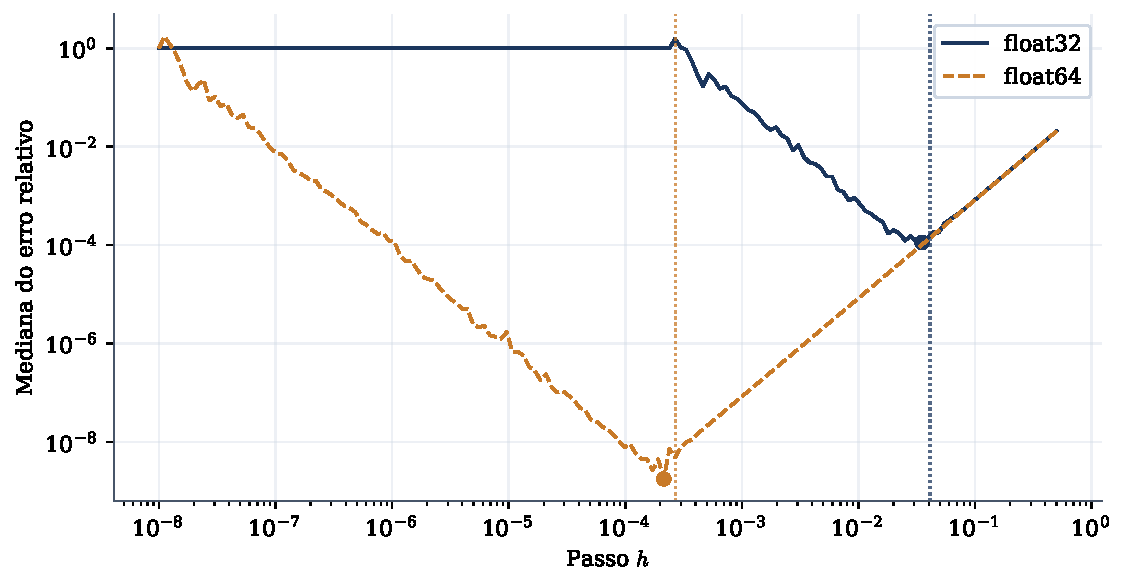
\includegraphics[width=0.75\textwidth]{figuras/notebook_original/a3.pdf}
\caption{Segunda derivada de $e^x$ pela parte real do passo complexo, em \texttt{float32} e \texttt{float64}: mediana do erro relativo em 65 abscissas. Verticais: $h^\ast$ do modelo.}
\label{fig:a3}
\end{figure}

\paragraph{O que isso diz sobre os limites do truque.} O passo complexo funciona para $f'$ por uma razão estrutural: a parte imaginária começa no termo de interesse, $hf'(x)$, sem nenhum termo $O(1)$ a ser removido. Para a parte real, o termo de interesse $h^2f''/2$ está atrás de $f(x)$, e removê-lo exige subtrair. Um passo inclinado $\omega=e^{\mathrm i\pi/4}$ ($\omega^2=\mathrm i$) leva $f''$ para a parte imaginária, $\Im[f(x+\omega h)+f(x-\omega h)]/h^2 = f''(x)-\frac{h^4}{360}f^{(6)}(x)+\cdots$~\cite{lai2008}; ainda há cancelamento, mas de termos $O(h)$, e por isso o erro melhora muito sem chegar a $u$. Para derivadas de ordem superior sem cancelamento são necessárias várias unidades imaginárias independentes (números multicomplexos) ou, no lado da AD, hiperduais $a+b\varepsilon_1+c\varepsilon_2+d\varepsilon_1\varepsilon_2$ ($\varepsilon_1^2=\varepsilon_2^2=0$, equivalentes a um dual de duais): com $x=x_0+\varepsilon_1+\varepsilon_2$, o coeficiente de $\varepsilon_1\varepsilon_2$ é $f''(x_0)$. Não há $h$, e portanto nem truncamento nem cancelamento.


%======================================================================
\section{Implementação (B1)}
\label{sec:impl}

A classe \texttt{Dual} guarda \texttt{val} (valor, um real finito) e \texttt{der} (derivada, escalar ou vetor) e sobrecarrega os operadores aritméticos com as regras da Seção~\ref{sec:dual}. Trecho central:

\begin{lstlisting}
class Dual:
    def __init__(self, val, der=0.0):
        self.val = real_finito(val, "val")     # parte real: valor
        self.der = np.array(der, dtype=float)  # parte dual: derivada(s)

    # produto: (a+bε)(c+dε) = ac + (ad+bc)ε  (regra do produto)
    def __mul__(self, other):
        other = Dual.converter(other)
        return Dual(self.val * other.val,
                    self.der * other.val + self.val * other.der)

    # quociente sem formar c²: (a/c, (a' - (a/c)c') / c)
    def __truediv__(self, other):
        other = Dual.converter(other)
        valor = self.val / other.val
        return Dual(valor, (self.der - valor * other.der) / other.val)

    def __abs__(self):          # sem derivada em 0: sinaliza
        if self.val == 0:
            raise ValueError("abs em zero")
        return Dual(abs(self.val), np.sign(self.val) * self.der)

# regra da cadeia: g(a+bε) = g(a) + g'(a)·b·ε
def aplicar(x, g, dg):
    if isinstance(x, Dual):
        return Dual(g(x.val), dg(x.val) * x.der)
    return g(x)

def exp(x): return aplicar(x, np.exp, np.exp)
def sin(x): return aplicar(x, np.sin, np.cos)
\end{lstlisting}

Três decisões de projeto merecem destaque:
\begin{enumerate}
\item \textbf{Validação em vez de convenção.} Valores e derivadas precisam ser reais finitos, e os pontos sem derivada real finita (\texttt{abs} em $0$, \texttt{log} de não positivo, $0^p$ com $p<1$) levantam exceção em vez de devolver uma derivada lateral. As funções \texttt{exp}, \texttt{sin}, \texttt{cos}, \texttt{log} aceitam \texttt{float}, \texttt{complex}, arrays e \texttt{Dual}, de modo que cada função de teste é escrita uma única vez.
\item \textbf{Sementes vetoriais.} Para gradientes, \texttt{der} pode ser um vetor de $n$ derivadas. Um array \texttt{dtype=object} com $x_i+e_i\varepsilon$ propaga as $n$ derivadas parciais numa só passada (Seção~\ref{sec:c2}).
\end{enumerate}

As funções pedidas são, sem as validações,
\begin{lstlisting}
def deriv_complexa(f, x, h=1e-30):
    return np.imag(f(x + 1j * h)) / h

def deriv_dual(f, x):
    return float(Dual.converter(f(Dual(x, 1.0))).der)
\end{lstlisting}

%======================================================================
\section{Passo complexo $\times$ duais em cinco funções (B2)}

A Tabela~\ref{tab:b2} resume os testes.

\begin{table}[h]
\centering\small
\begin{tabular}{p{4.8cm}p{4.2cm}p{4.6cm}}
\toprule
Função & Passo complexo & Dual \\
\midrule
1. $e^x$, $x=1$ & erro rel.\ $0$ & erro rel.\ $0$ \\
2. $\log x$, $x=2$ & erro rel.\ $0$ & erro rel.\ $0$ \\
3. $e^{\sin x^2}$, $x=0{,}7$ & erro rel.\ $2{,}2\times10^{-16}$ & erro rel.\ $0$ \\
4. $|x|$, $x=\pm1$ & \textbf{falha}: $0$ (correto: $\pm1$) & correto \\
\phantom{4.} $|x|$, $x=0$ (não diferenciável) & $0$, sem aviso & \texttt{ValueError} \\
5. $[A(x)^{-1}r]_1$, $A=\left(\begin{smallmatrix}2&x\\1&3\end{smallmatrix}\right)$, via \texttt{np.linalg.solve}, $x=1$ & erro rel.\ $1{,}5\times10^{-16}$ & \textbf{falha} (\texttt{dtype=object}) \\
\bottomrule
\end{tabular}
\caption{Resultados de \texttt{deriv\_complexa} e \texttt{deriv\_dual} (notebook, B2).}
\label{tab:b2}
\end{table}

\paragraph{Funções 1--3.} Ambos atingem $\sim u$.

\paragraph{Função 4: \texttt{abs}.} Para complexos, \texttt{abs} calcula o módulo $\sqrt{\Re^2+\Im^2}$, que é real: a parte imaginária, que transportava a derivada, é apagada e $|x|$ passa a ser tratado como constante. O passo complexo devolve $0$ \emph{mesmo longe do ponto singular}, sem aviso. A correção de Martins et al.~\cite{martins2003} é redefinir $\mathrm{abs}(z) = -z$ se $\Re z<0$ e $z$ caso contrário. Em $x=0$ a derivada não existe: o passo complexo devolve $0$ em silêncio, enquanto a nossa \texttt{Dual} levanta \texttt{ValueError}. Outras armadilhas do mesmo tipo: \texttt{max}/\texttt{min} e comparações com a parte imaginária, conjugação (por exemplo \texttt{np.vdot}, ou $x\bar x$ em vez de $x^2$), e funções implementadas via módulo complexo.

\paragraph{Função 5: \texttt{np.linalg.solve}.} O passo complexo funciona porque o LAPACK tem rotinas complexas (\texttt{zgesv}), e a extensão analítica de $x\mapsto A(x)^{-1}r$ é justamente a inversão em aritmética complexa. Já o \texttt{Dual} falha: o \texttt{solve} converte a entrada num \texttt{ndarray} numérico, e uma matriz de \texttt{Dual}s (\texttt{dtype=object}) não é um tipo que o código compilado conheça. A saída é fornecer uma \emph{regra de derivada para a rotina inteira}: de $My=r$ segue $M\,\mathrm dy = \mathrm dr - \mathrm dM\,y$, ou seja, um segundo \texttt{solve} com a mesma matriz. É assim que PyTorch e JAX tratam álgebra linear: o \texttt{autograd} traz uma regra pronta para o \texttt{solve}, em vez de derivar o LAPACK por dentro.

\paragraph{Programas, não funções.} Expressões como $\sqrt{x^2}$ têm derivada AD indefinida em $x=0$ ($0/0$ na regra da cadeia de $\sqrt{\cdot}$), embora $\sqrt{x^2}=|x|$. Um método iterativo dentro de $f$ é derivado através das iterações, e o resultado depende do critério de parada.

%======================================================================
\section{Erro em função de $h$ (C1)}

A Figura~\ref{fig:c1} mostra o erro absoluto de $f'(1{,}5)$ para $f(x)=e^x/(\cos^3x+\sin^3x)$, com $h\in[10^{-20},10^{-1}]$ e referência com 60 dígitos (\texttt{mpmath}). As verticais tracejadas são os $h^\ast$ do modelo; a pontilhada marca o início do patamar do passo complexo. Todas as fórmulas usam o passo efetivo $(x+h)-x$, que elimina o erro extra $u|x|/h$ do arredondamento de $x+h$. A Tabela~\ref{tab:c1} compara teoria e experimento. Como a curva é ruidosa onde domina o arredondamento, comparamos o erro previsto com a mediana dos 7 pontos da malha mais próximos de $h^\ast$; o menor erro da malha é um cancelamento fortuito.

\begin{figure}[h]
\centering
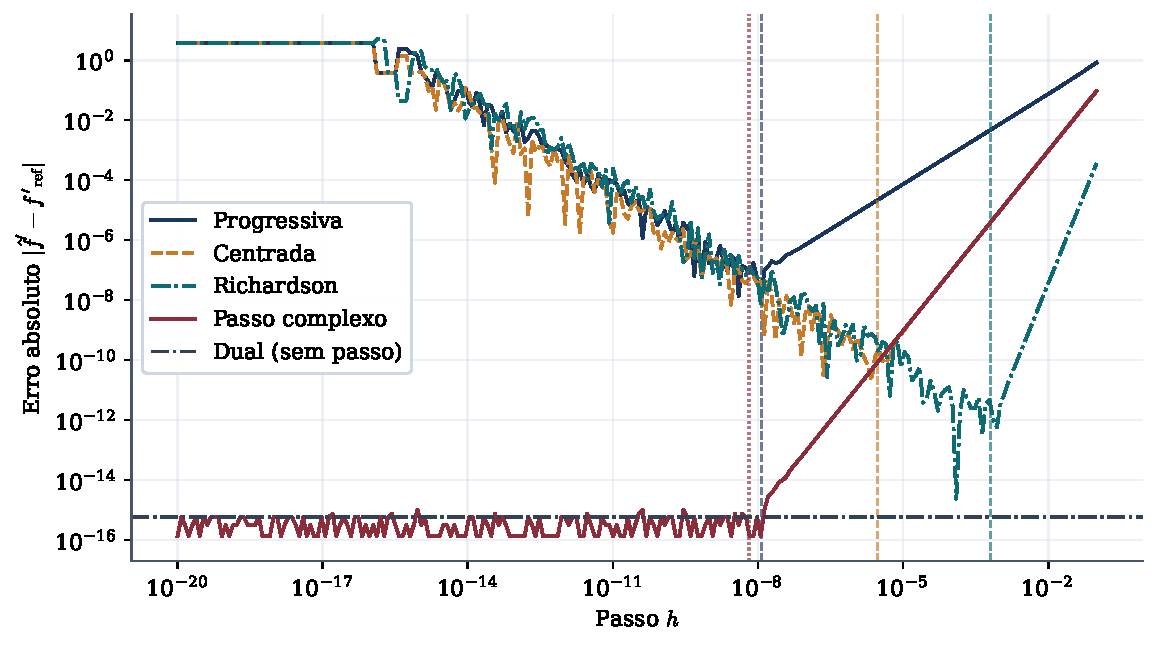
\includegraphics[width=0.9\textwidth]{figuras/notebook_original/c1.pdf}
\caption{Erro absoluto $\times$ $h$. A horizontal é o erro da \texttt{Dual}, que não tem passo.}
\label{fig:c1}
\end{figure}

\begin{table}[h]
\centering\small
\setlength{\tabcolsep}{3pt}\begin{tabular}{lccccc}
\toprule
Método & $p$ & $h^\ast$ (modelo) & erro previsto & mediana perto de $h^\ast$ & mínimo da malha \\
\midrule
progressiva & 1 & $1{,}2\times10^{-8}$ & $1{,}7\times10^{-7}$ & $9{,}8\times10^{-8}$ & $9{,}7\times10^{-9}$ \\
centrada & 2 & $3{,}0\times10^{-6}$ & $2{,}5\times10^{-10}$ & $9{,}5\times10^{-11}$ & $2{,}0\times10^{-11}$ \\
Richardson & 4 & $6{,}4\times10^{-4}$ & $2{,}9\times10^{-12}$ & $3{,}3\times10^{-12}$ & $2{,}4\times10^{-15}$ \\
passo complexo & 2 & $h\lesssim6{,}5\times10^{-9}$ & $u|f'|=4{,}0\times10^{-16}$ & $3{,}1\times10^{-16}$ & $1{,}3\times10^{-16}$ \\
dual & --- & --- & $\sim u|f'|$ & \multicolumn{2}{c}{$5{,}8\times10^{-16}$ (sem passo)} \\
\bottomrule
\end{tabular}
\caption{Passos ótimos e erros absolutos em $f'(1{,}5)=3{,}622$. O menor erro de Richardson é um cancelamento fortuito; a mediana segue o modelo.}
\label{tab:c1}
\end{table}

À direita de cada mínimo domina o truncamento (inclinação $p$); à esquerda, o cancelamento (inclinação $-1$). As três curvas de diferenças finitas compartilham, a menos de constantes, a mesma perna esquerda $u|f|/h$: aumentar a ordem só abaixa o vértice do ``V''. Para $h<u|x|\approx 3\times10^{-16}$ as diferenças finitas devolvem zero. O passo complexo tem a mesma perna direita que a centrada, mas a perna esquerda simplesmente não existe.

%======================================================================
\section{Gradiente em $\mathbb{R}^{100}$ (C2)}
\label{sec:c2}

Para $f(x)=\frac12x^\top Ax-b^\top x$ com $A=M^\top M/n+I$ simétrica ($M$ aleatória, semente 42), $\nabla f(x)=Ax-b$. A Tabela~\ref{tab:c2} mostra o erro relativo em norma euclidiana e o tempo (mediana de 5 execuções após aquecimento). A \texttt{Dual} vetorizada é um array \texttt{dtype=object} com um \texttt{Dual} por coordenada, cada um carregando as 100 derivadas. Os tempos absolutos dependem da máquina.

\begin{table}[h]
\centering
\begin{tabular}{lccc}
\toprule
Método & avaliações & erro rel.\ ($\|\cdot\|_2$) & tempo (ms) \\
\midrule
diferenças centradas & 200 reais & $5{,}8\times10^{-10}$ & $15$ \\
passo complexo & 100 complexas & $2{,}4\times10^{-16}$ & $73$ \\
\texttt{Dual} vetorizada & 1 (com 100 direções) & $3{,}6\times10^{-16}$ & $359$ \\
\texttt{torch.func.jacfwd} (direto) & 1 (vetorizada) & $9{,}5\times10^{-17}$ & --- \\
\texttt{torch.func.grad} (reverso) & 1 direta + 1 reversa & $1{,}9\times10^{-16}$ & --- \\
\bottomrule
\end{tabular}
\caption{Gradiente em $\mathbb{R}^{100}$. Tempos de uma execução do notebook; as linhas do PyTorch vêm de D1, que não mede tempo.}
\label{tab:c2}
\end{table}

\begin{figure}[H]
\centering
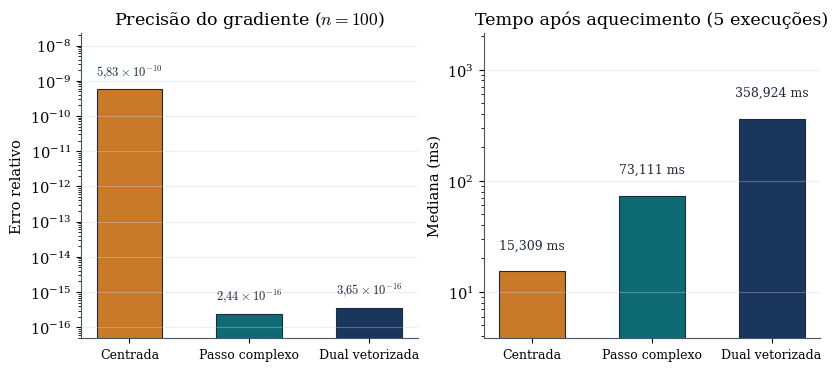
\includegraphics[width=0.85\textwidth]{figuras/notebook_original/c2_colega.png}
\caption{Precisão e tempo dos métodos genéricos em $\mathbb R^{100}$.}
\label{fig:c2-barras}
\end{figure}

Como $f$ é quadrática, $f'''\equiv0$ e a diferença centrada não tem erro de truncamento: os $6\times10^{-10}$ observados são \emph{puro cancelamento}. Para confirmar, somamos $\sum_i\sin x_i$ à quadrática e repetimos os mesmos passos (Figura~\ref{fig:c2b}): na quadrática o erro cai até $3{,}3\times10^{-15}$ com $h=1$; com os senos volta o ``V'', com mínimo $1{,}6\times10^{-10}$ em $h\approx3\times10^{-5}$ e erro $7{,}7\times10^{-2}$ em $h=1$.

\begin{figure}[H]
\centering
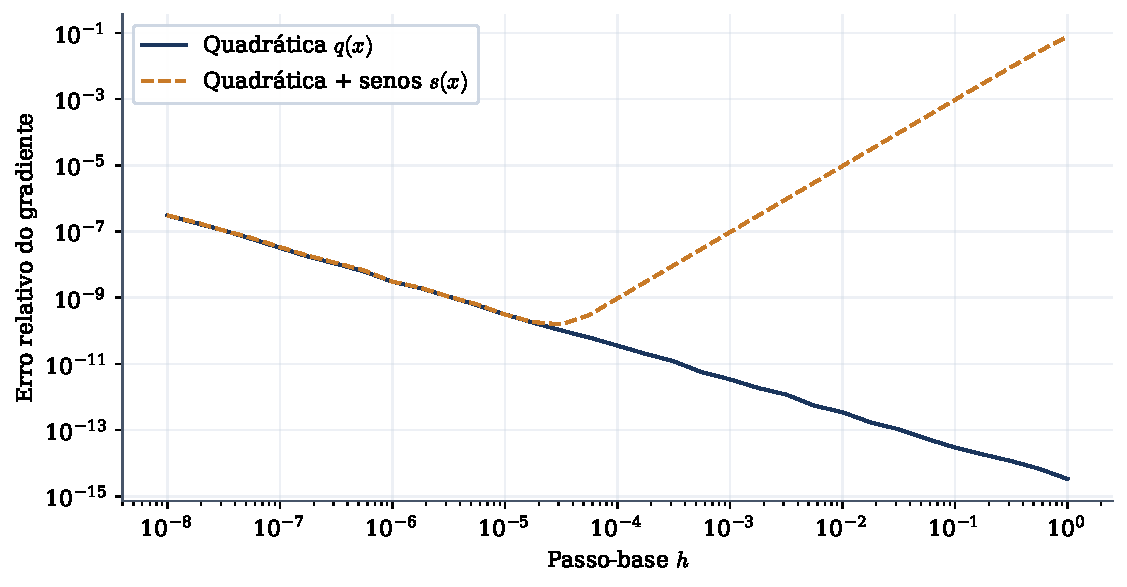
\includegraphics[width=0.75\textwidth]{figuras/notebook_original/c2b.pdf}
\caption{Erro do gradiente por diferenças centradas em função do passo-base, com e sem termo não quadrático.}
\label{fig:c2b}
\end{figure}

\paragraph{Custo $O(n)$ do modo direto.} Diferenças finitas, passo complexo e duais calculam, a cada avaliação, uma única \emph{derivada direcional} $\nabla f(x)\cdot v$. O gradiente exige as $n$ direções $e_1,\dots,e_n$, logo
\[
\text{custo}(\nabla f) \approx n\cdot \text{custo}(f)\quad(\text{ou }2n\text{ para a centrada}).
\]
A \texttt{Dual} com sementes vetoriais não escapa disso: faz uma só passada, mas cada número carrega $n$ derivadas, e o produto $Ax$ passa de $n^2$ operações a $n^3$. Em operações, portanto, a \texttt{Dual} não é mais barata que o passo complexo: os dois custam $O(n^3)$ aqui. O que decide o relógio é a implementação. Na nossa \texttt{Dual}, cada uma das $n^2$ multiplicações de $Ax$ passa por um objeto Python, e ela fica cerca de 5 vezes mais lenta que o passo complexo; isso é custo do interpretador, não do método. Uma \texttt{Dual} cujo valor também fosse um array NumPy faria $Ax$ como produto matriz$\times$matriz no BLAS e seria muito mais rápida, mas o fator $n$ em operações continuaria lá. O passo complexo paga ainda um fator constante extra: uma multiplicação complexa custa cerca de 4 reais.

\paragraph{Custo $O(1)$ do modo reverso.} O modo reverso percorre o programa duas vezes. Na ida, avalia $f$ e grava numa ``fita'' as operações e valores intermediários. Na volta, propaga \emph{adjuntos} $\bar v_j=\partial f/\partial v_j$ da saída ($\bar f=1$) para as entradas, usando $\bar v_i \mathrel{+}= \bar v_j\,\partial\phi_j/\partial v_i$. Cada operação elementar gera um número constante de operações na volta; ao final, $\bar x = \nabla f(x)$ completo. Daí
\[
\text{custo}(\nabla f)\le c\cdot\text{custo}(f),\qquad c\approx 3\text{ a }5,
\]
independente de $n$ (o ``princípio do gradiente barato''~\cite{baydin2018,griewank2008}). Em termos de álgebra linear: o modo direto calcula produtos Jacobiano$\times$vetor $J v$, um por coluna; o reverso calcula $v^\top J$, um por linha. Para $f:\mathbb{R}^n\to\mathbb{R}$, $J$ tem $n$ colunas e uma só linha. O custo do reverso é memória: a fita cresce com o número de operações.

%======================================================================
\section{Modos direto e reverso em JAX e PyTorch (C3, D1)}

Em JAX (\texttt{float64}), o gradiente da quadrática de C2 tem erro relativo $1{,}6\times10^{-16}$ pelo modo direto (\texttt{jax.jacfwd}) e $1{,}7\times10^{-16}$ pelo reverso (\texttt{jax.grad}). Com JIT, a mediana após aquecimento foi $0{,}23$\,ms no direto e $0{,}03$\,ms no reverso, cerca de 8 vezes menos (Figura~\ref{fig:c3}). Sem JIT explícito, os dois ficam em 4 a 5\,ms, dominados pelo despacho. Tempos dessa ordem são sensíveis à máquina e à carga, e com $n=100$ só, isso ilustra a diferença entre os modos, mas não estima expoente.

Em PyTorch, \texttt{torch.func.grad}, \texttt{backward()} e \texttt{torch.func.jacfwd} concordam com $Ax-b$ e com o JAX no nível de $u$ (diferenças máximas de $1{,}3\times10^{-15}$, vindas da ordem das somas). Na derivada de $e^{\sin x^2}$ em $x=0{,}7$, \texttt{Dual}, passo complexo, JAX e PyTorch diferem da analítica em no máximo $4{,}4\times10^{-16}$.

\begin{figure}[H]
\centering
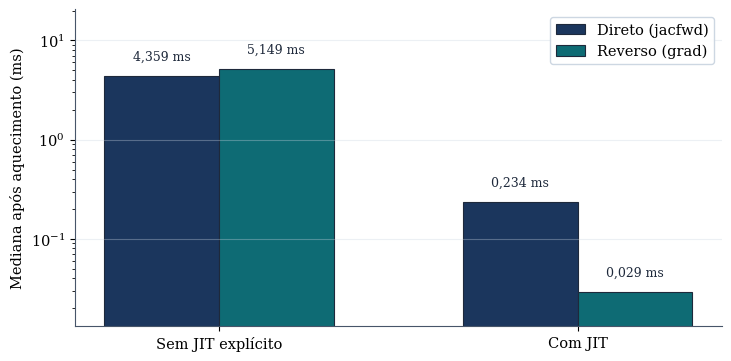
\includegraphics[width=0.7\textwidth]{figuras/notebook_original/c3_colega.png}
\caption{Gradiente da quadrática em JAX: mediana dos tempos após aquecimento, com e sem JIT.}
\label{fig:c3}
\end{figure}

Em pontos de não-diferenciabilidade, cada ferramenta adota uma convenção diferente:

\begin{center}
\begin{tabular}{lc}
\toprule
Cálculo de $\frac{\mathrm d}{\mathrm dx}|x|$ & resultado em $x=0$ \\
\midrule
\texttt{jax.grad(jnp.abs)} & $1$ \\
\texttt{torch.func.grad(torch.abs)} & $0$ \\
passo complexo com \texttt{abs} & $0$ \\
nossa \texttt{Dual} & \texttt{ValueError} \\
\bottomrule
\end{tabular}
\end{center}

O subdiferencial de $|x|$ em $0$ é $[-1,1]$, e qualquer valor nele é um subgradiente válido. O JAX cai no ramo positivo (derivada lateral à direita); o PyTorch usa $\operatorname{sign}(0)=0$, o subgradiente de norma mínima. O $0$ do passo complexo não é uma convenção: vem de \texttt{abs} apagar a parte imaginária, e aparece também longe da origem (Seção B2). A nossa \texttt{Dual} prefere sinalizar. A lição: \textbf{AD devolve a derivada exata do programa no ramo executado}; em pontos de quebra o resultado é uma convenção de implementação, não uma propriedade matemática de $f$.

%======================================================================
\section{Custo em generalidade e em implementação}

\begin{table}[h]
\centering\small
\begin{tabular}{p{2.6cm}p{2.5cm}p{2.9cm}p{2.9cm}p{2.5cm}}
\toprule
& Diferenças finitas & Passo complexo & AD direta (duais) & AD reversa \\
\midrule
Melhor erro & $u^{p/(p+1)}$ & $\sim u$ & $\sim u$ & $\sim u$ \\
Parâmetro $h$ & crítico & irrelevante ($h\ll\sqrt u$) & não há & não há \\
O que exige de $f$ & só avaliar (caixa-preta) & analítica; código \emph{complex-safe} & código em operações sobrecarregáveis & idem, mais fita \\
Código compilado & sim & se aceitar complexos & só com regra própria & só com regra própria \\
Mudança no código & nenhuma & trocar tipos para complexo; reescrever \texttt{abs}, \texttt{max}, comparações & trocar tipos para \texttt{Dual}; biblioteca de AD & biblioteca de AD \\
Gradiente em $\mathbb R^n$ & $n$ ou $2n$ aval. & $n$ aval.\ complexas & $n$ direções & $O(1)$ aval., memória $O(\#\text{ops})$ \\
2ª derivada & cancelamento & cancelamento volta & exata (aninhado) & exata (aninhado) \\
\bottomrule
\end{tabular}
\caption{Resumo comparativo.}
\end{table}

\paragraph{Generalidade.} Diferenças finitas aceitam qualquer $f$ que possa ser avaliada, inclusive executáveis de terceiros; essa é a sua grande virtude. O passo complexo exige que $f$ admita extensão analítica \emph{e} que o código a calcule corretamente: funções como $|x|$, $\max$, $\min$, comparações e conjugação precisam ser reescritas, e qualquer rotina que trate o complexo como módulo destrói a derivada em silêncio (função 4a). Em troca, atravessa código compilado que aceite complexos (função 5). Os duais aceitam funções apenas diferenciáveis (não precisam de analiticidade) e tratam \texttt{abs} e desvios de forma natural fora dos pontos de quebra, mas exigem que \emph{cada} operação passe pela sobrecarga: uma única chamada a código que não conhece o tipo quebra a cadeia (função 5), e a solução é escrever regras de derivada para rotinas inteiras.

\paragraph{Implementação.} Diferenças finitas: três linhas, mais o problema de escolher $h$. Passo complexo: uma linha, mais a auditoria do código para trocar \texttt{float} por \texttt{complex} e reescrever as funções não analíticas; em Fortran/C isso pode ser automatizado por scripts~\cite{martins2003}. Duais: uma classe com algumas dezenas de linhas resolve o caso escalar, mas uma ferramenta robusta exige cobrir toda a biblioteca matemática, álgebra linear e controle de memória. O modo reverso é o mais complexo de implementar (fita, ordem reversa, gerenciamento de memória), e é por isso que se usam bibliotecas como PyTorch e JAX.

%======================================================================
\section{Conclusão}

\begin{enumerate}
\item \textbf{Por que diferenças finitas nunca atingem $u$:} toda fórmula exata para constantes precisa subtrair valores próximos de $f$; essa subtração transforma o erro absoluto $u|f|$ em um erro $u|f|/h$ na derivada, e o equilíbrio com o truncamento $Ch^p$ limita o erro a $u^{p/(p+1)}$.
\item \textbf{O que o passo complexo faz:} desloca a perturbação para uma direção ``ortogonal'' (a parte imaginária), onde a derivada aparece isolada como termo principal. Sem subtração, sem $u/h$; o truncamento $O(h^2)$ some escolhendo $h$ minúsculo.
\item \textbf{O que a AD faz:} substitui $\mathrm i^2=-1$ por $\varepsilon^2=0$, o que torna a série de Taylor finita e elimina também o truncamento. Cada operação aplica a regra de derivação exata e o único erro é o arredondamento da própria aritmética.
\item \textbf{O custo:} o passo complexo troca generalidade (analiticidade, código \emph{complex-safe}) por facilidade de uso em código existente; a AD troca generalidade de \emph{implementação} (tudo precisa passar pela sobrecarga ou ter regra própria) por exatidão e pela possibilidade do modo reverso, o único que calcula gradientes em $\mathbb R^n$ a custo $O(1)$ avaliações. Nenhum dos dois resolve pontos de não-diferenciabilidade: as bibliotecas devolvem, em silêncio, uma derivada lateral ou um subgradiente convencional, e uma implementação própria pode, no máximo, sinalizar o ponto.
\end{enumerate}

%======================================================================
\begin{thebibliography}{9}
\bibitem{squire1998} W.~Squire e G.~Trapp. Using complex variables to estimate derivatives of real functions. \emph{SIAM Review}, 40(1):110--112, 1998.
\bibitem{martins2003} J.~R.~R.~A. Martins, P.~Sturdza e J.~J. Alonso. The complex-step derivative approximation. \emph{ACM Transactions on Mathematical Software}, 29(3):245--262, 2003.
\bibitem{baydin2018} A.~G. Baydin, B.~A. Pearlmutter, A.~A. Radul e J.~M. Siskind. Automatic differentiation in machine learning: a survey. \emph{Journal of Machine Learning Research}, 18(153):1--43, 2018.
\bibitem{griewank2008} A.~Griewank e A.~Walther. \emph{Evaluating Derivatives: Principles and Techniques of Algorithmic Differentiation}. 2.\,ed., SIAM, 2008.
\bibitem{higham2002} N.~J. Higham. \emph{Accuracy and Stability of Numerical Algorithms}. 2.\,ed., SIAM, 2002.
\bibitem{lai2008} K.-L. Lai e J.~L. Crassidis. Extensions of the first and second complex-step derivative approximations. \emph{Journal of Computational and Applied Mathematics}, 219(1):276--293, 2008.
\end{thebibliography}

\end{document}
